\chapter{Lastimpedantie-analyse}
\label{loadanalysis}
Om een cel uit te lezen wordt er een spanning gevormd op de bitline door middel van een spanningsdeling.
Het is dus belangrijk om de 2 impedanties van de spanningsdeler zodanig te kiezen voor optimale snelheid, bitline spanningsverschil en spanningsval over de memristor.
Ook belangrijk is dat deze impedanties robuust zijn tegen variabiliteit.

\section{Algemene lasteigenschappen en -specificaties}\label{sec:simplemodel}
In deze eerste sectie bestuderen we de combinatie van last en memristor cell als een heel simpel model namelijk twee weerstanden in serie (zie figuur \ref{fig:simplemodel}). Dit om aan te tonen dat de weerstands waarde van de last een grote invloed heeft op de het spanningsverschil tussen een hoge en lage celweerstand, bitlijn snelheid en de gevoeligheid van beide.
Het verschil in bitlijn voltage tussen een hoge en lage cell is van belang voor de tolleranties op de referentiespanning en sense amplifier mismatch. In het simpele model kan het verschil in bitlijn voltage analytisch berekend worden met de volgende formule:
\begin{equation}
 \Delta V = \frac{R_{HRS}}{R_{last}+R_{HRS}} - \frac{R_{LRS}}{R_{last}+R_{LRS}}
\end{equation} 
Voor constante waarden van $R_{HRS}$ en $R_{LRS}$ is er een maximum in $ \Delta V$ zoals duidelijk gezien kan worden op figuur \ref{fig:rpiek}. De sensitiviteit van de last weerstand op het spanningsverschil moet men voorzichtig interpreteren. Op figuur \ref{fig:rpiek} kan gezien worden dat de helling voor het maximum stijler is dan voorbij het maximum. Het is dus beter om een iets grotere weerstand te hebben dan een iets te kleine weerstand. Maar als men deze weerstand naar transistorafmetingen vertaalt, kan met dit op verschillend manieren realiseren. De aanweerstand van een transistor is omgekeerd evenredig met $\frac{W}{L}$ en proportioneel met L. Voor een transistor met minimale lengte kan de grootste aanweerstand dus enkel gerealiseerd worden voor minimale breedte. Dit is gevoeliger voor mismatch dan transistoren met grotere breedtes.\\
De snelheid van het opladen van de bitlijn kan in het simpele model ook analytisch beschreven worden. De volgende vergelijking stelt de tijd voor wanneer de bitlijn $99\%$ is opgeladen.

\begin{align}
t = -ln(0.01)*RC\\
R^{-1} = \frac{1}{R_{cell}} + \frac{1}{R_{last}}
\end{align}

Deze tijd zal kleiner worden als R kleiner wordt, dit vertaalt zich dan naar een kleine lastimpedantie.

\begin{figure}[!ht]
\centering
\subfloat[het simpel bitlijn model]{ 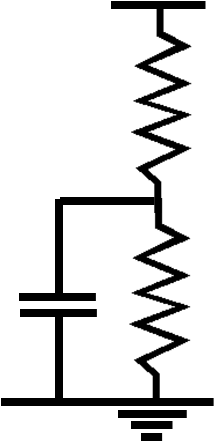
\includegraphics[width=0.20\textwidth] {../fig/hfdst-last-simplemodel.png} \label{fig:simplemodel}}
\subfloat[Verschil in bitlijnspanning in functie van lastweerstand]{ 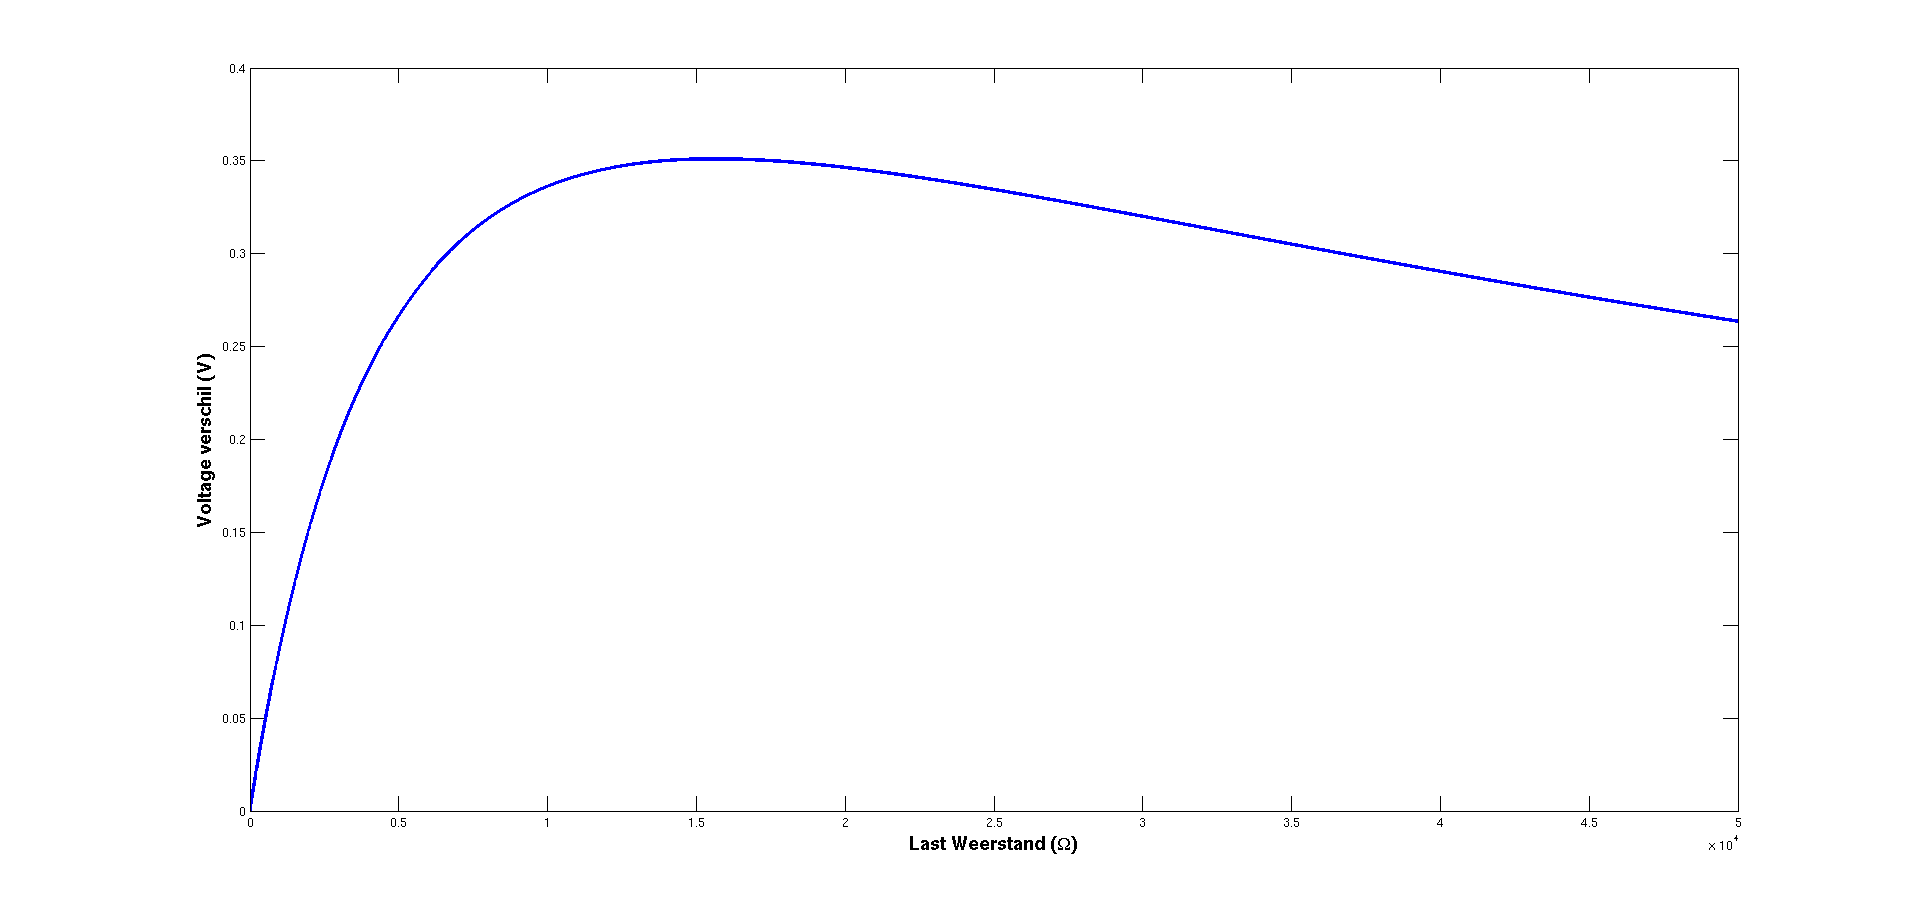
\includegraphics[width=0.80\textwidth] {../fig/hfdst-last-rpiek.png} \label{fig:rpiek}}
\caption{}
\end{figure}




\section{Evalueren van de last}
Om verschillende lasten met elkaar te kunnen vergelijken, is het belangrijk om hun eigenschappen allemaal op dezelfde manier te bekomen. Figuur \ref{fig:simsetup} geeft de verschillende aspecten van de gebruikte simulatiesetup weer. Het testcircuit (figuur \ref{fig:simcircuit}) stelt een bitlijn voor met een capaciteit van 18fF, wat ruwweg overeenkomt met een bitlijn waaraan 100 cellen hangen. Aan deze bitlijn zijn naast de cel ook een last en een ontladinstransistor aangesloten. De ontladingstransistor is minimaal gehouden. De memristor weerstand kan de volgende waardes hebben: tussen 5k$\Omega$ en 10k$\Omega$ voor de LRS, tussen de 30k$\Omega$ en 35k$\Omega$ voor de HRS. De nominale waardes voor LRS en HRS zijn 7.5k$\Omega$ en 32.5k$\Omega$. Tijdens Monte Carlo simulaties worden deze nominale waardes als verwachtingswaarde genomen van een gausische distributie met $\sigma = 0.833k\Omega$. Aan deze memristor weerstand hangt een WL-transistor, die ook minimaal gehouden wordt. De combinatie van deze wordt de geheugencel genoemd. De cel hangt aan de BL, WL en SL. Aan de SL is tenslotte nog een ontladingstransistor verbonden. Deze transistor werd bewust groot gemaakt zodat de equivalente weerstand van de onderste tak gedomineerd wordt door de weerstand van de geheugencel. Aan deze sourcelijn werd er ook een capaciteit van 18fF gehangen, al kan de invloed hiervan verwaarloosd worden, de ontladingstransistor aan de SL staat tenslotte altijd aan. Tenslotte wordt de voedingsspanning altijd op 1V gehouden.\\\\
Figuren \ref{fig:simcontr1} tot \ref{fig:simcontr3} stellen de sequentie voor van alle controlesignalen tijdens de simulatie. Eerst wordt de bitlijn volledig ontladen (figuur \ref{fig:simcontr1}). Vervolgens is er een interval waarin niet gebeurt (figuur \ref{fig:simcontr2}) en tenslotte wordt de last aangesloten en de bitlijn opgeladen (figuur \ref{fig:simcontr3}). De simulatie stopt wanneer de bitlijn volledig opgeladen is.\\

\begin{figure}[!ht]
\centering
\subfloat[Test circuit]{ 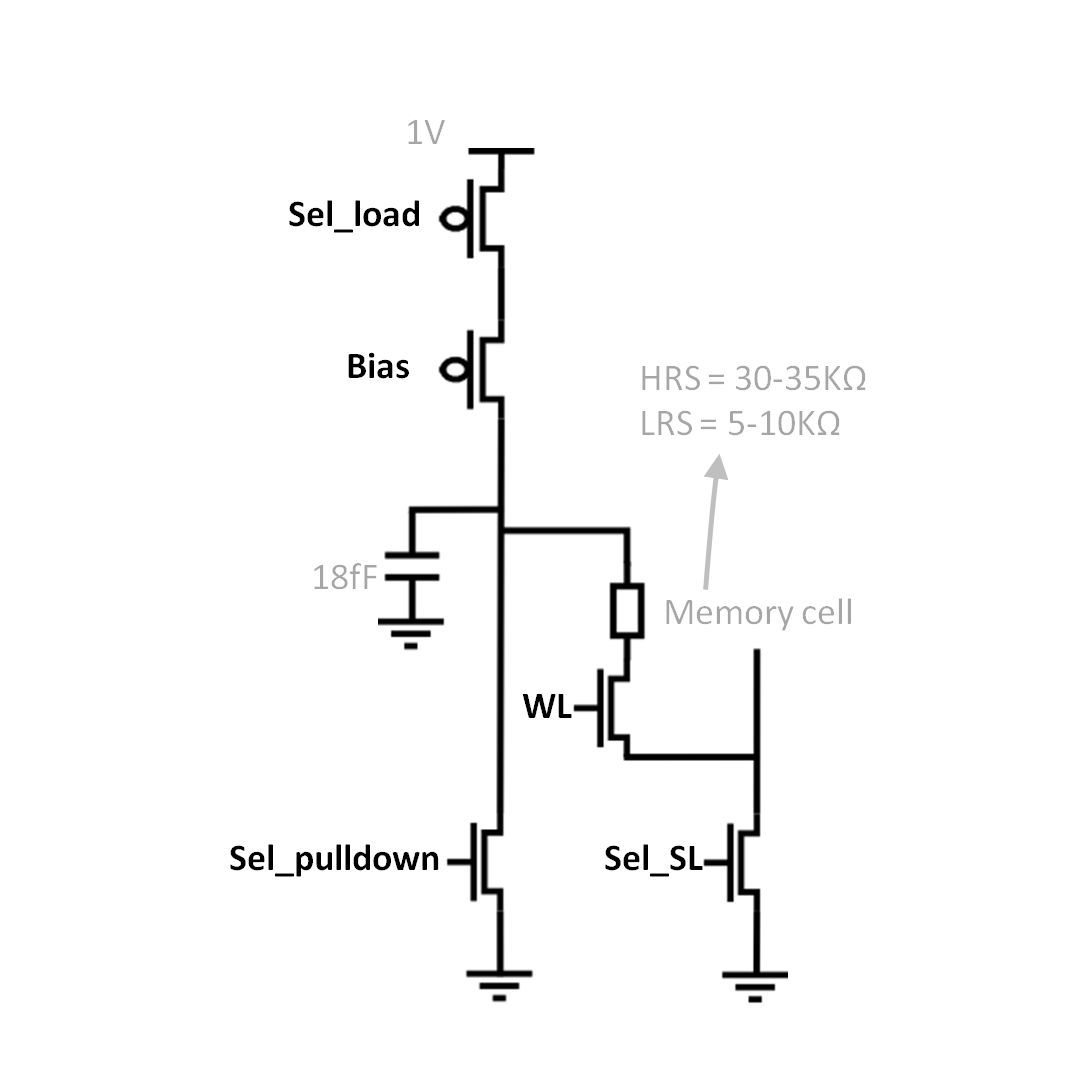
\includegraphics[width=0.45\textwidth] {../fig/hfdst-last-simsetup.png} \label{fig:simcircuit}}
\subfloat[Controle signalen 1]{ 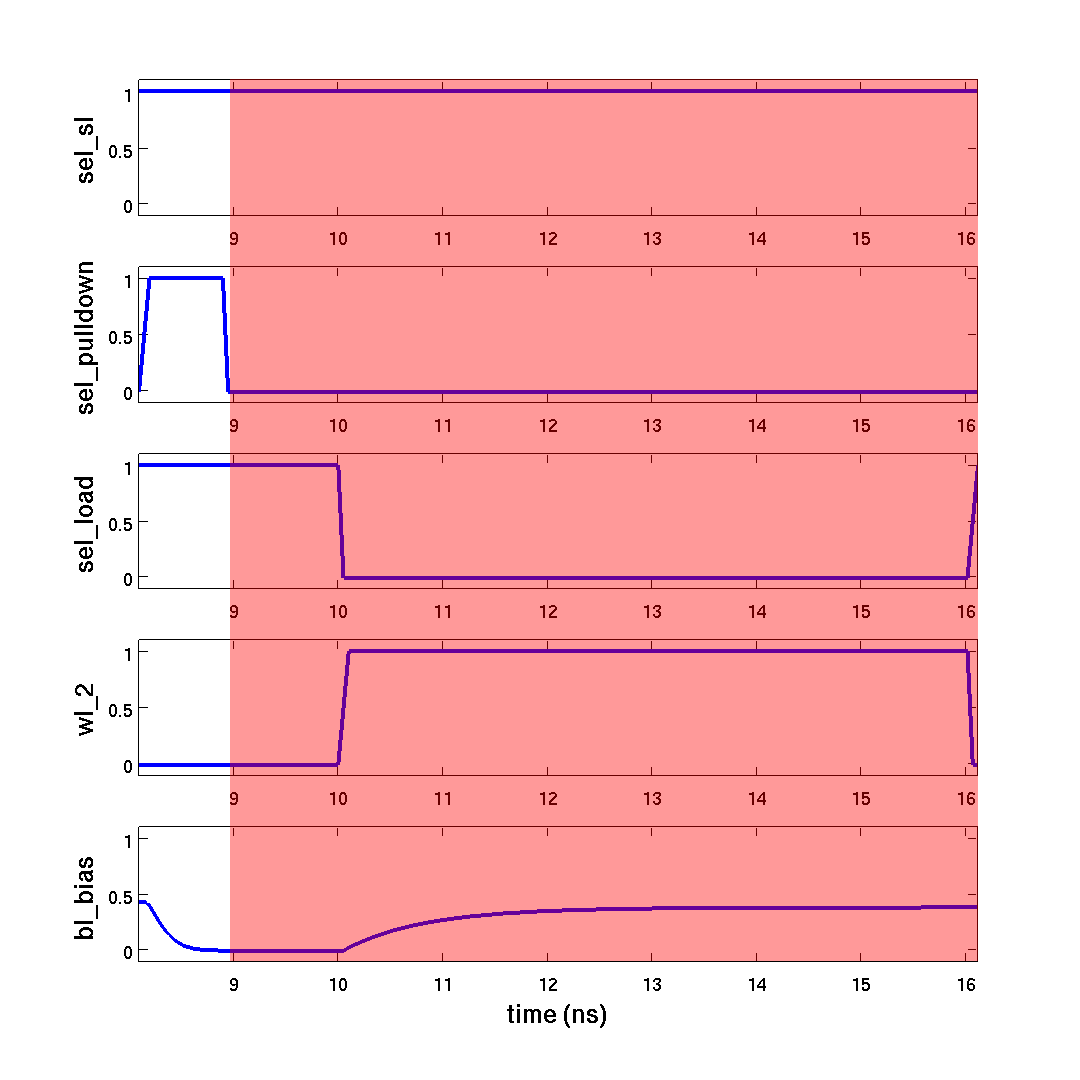
\includegraphics[width=0.45\textwidth] {../fig/hfdst-last-controlsig1.png} \label{fig:simcontr1}}\\
\subfloat[Controle signalen 2]{ 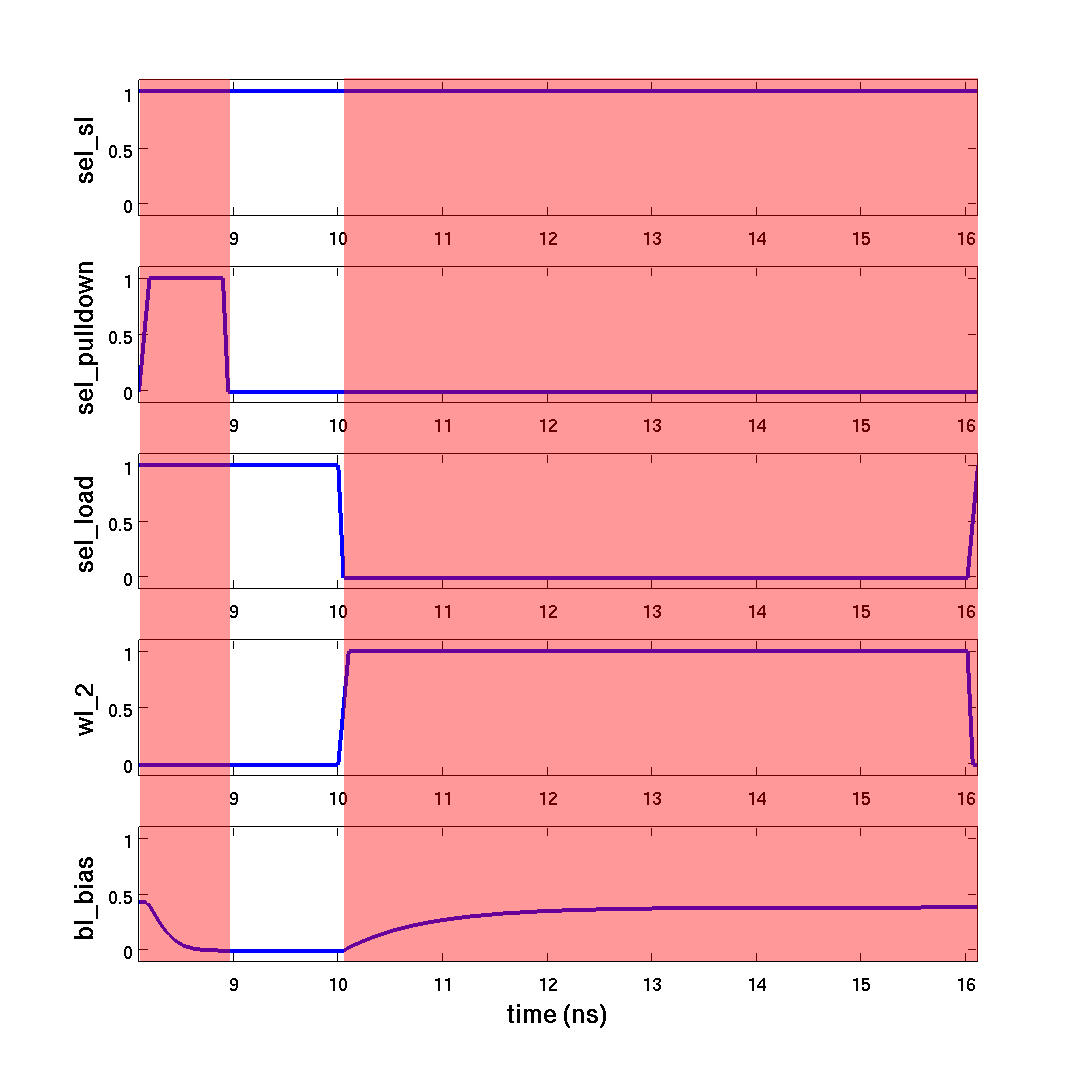
\includegraphics[width=0.45\textwidth] {../fig/hfdst-last-controlsig2.png} \label{fig:simcontr2}}
\subfloat[Controle signalen 3]{ 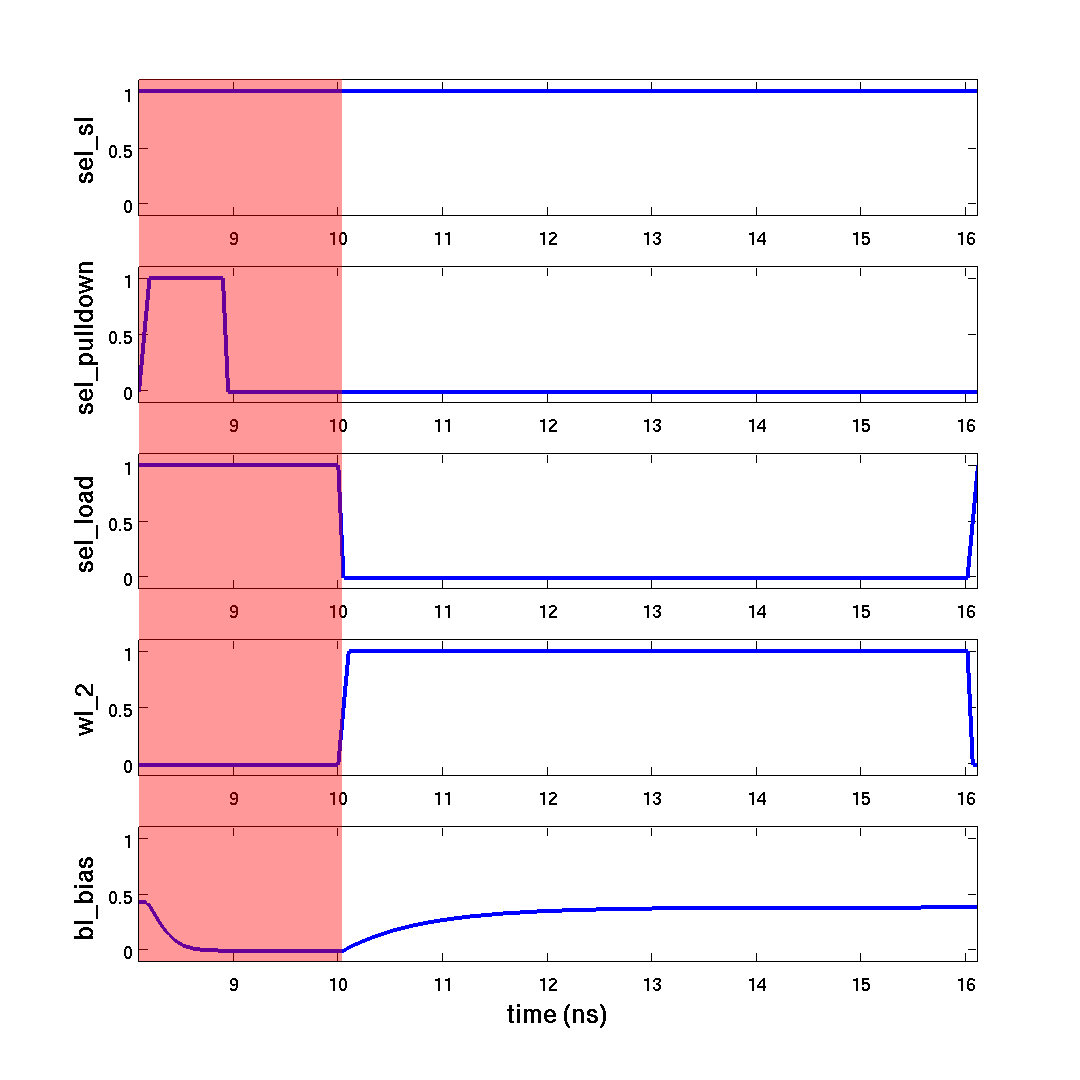
\includegraphics[width=0.45\textwidth] {../fig/hfdst-last-controlsig3.png} \label{fig:simcontr3}}
\caption{Testbench voor de lastimpedantie}\label{fig:simsetup}
\end{figure}

Eens een last gesimuleerd is wordt deze beoordeeld op vlak van oppervlakte, BL-laadsnelheid, nominaal BL-spanningsverschil en spanningsval over het geheugenelement. Het oppervlakte wordt berekend op basis van de lengtes en breedtes van de lasttransistoren. De BL-laadsnelheid is de tijd die nodig is om de bitlijn $99\%$ op te laden. Het nominale BL-spanninsverschil is het verschil van de spanning over 2 BLs - aan de ene hangt een cel in HRS, de andere een cel in LRS - wanneer de bitlijn $100\%$ opgeladen is. De bitlijn wordt verondersteld $100\%$ opgeladen te zijn op het einde van de simulatie en de simulatietijd word voldoende hoog gehouden om dit te garanderen. De spanningsval over het geheugenelement is belangrijk wat betreft destructieve leesoperaties. Een te grote spanning gedurende een te lange tijd zou een schakeling van resistieve toestand kunnen opwekken. De numerieke waarde van de maximale spanningsval over de cel is heel erg afhankelijk van het type memristor. In dit onderzoek wordt er gewerkt met een maximum van 0.5V over de cell \cite{ppt:model}.

\section{vergelijking van verschillende types last}
Voor dit onderzoek worden vier mogelijke kandidaten van lastimpedanties vergeleken: de switchload (figuur \ref{fig:switchload}), de biasload (figuur \ref{fig:biasload}), de diodeload (figuur \ref{fig:diodeload}) en de bulkload (figuur \ref{fig:bulkload})\cite{bulkload}. Eerst wordt er een lineare sweep gedaan op de verschillende lasten (sectie \ref{sec:linload}), waarbij enkel de breedtes en bias spanningen worden gesweept. De lengtes van de transistoren worden minimaal gehouden om er voor te zorgen dat de transistoren binnen de pitch van de bitlijn passen. Eens variabiliteit wordt toegevoegd aan de simulatie met Monte Carlo simulaties (sectie \ref{sec:varload}) zal echter blijken dat het verschil in BL-spanning te klein is en zal de lengte van de lasttransistoren ook moeten worden vergroot (sectie \ref{sec:finaleload}).

\begin{figure}[!ht]
  \centering
  \subfloat[De switch load]{\makebox[.22\textwidth]{ 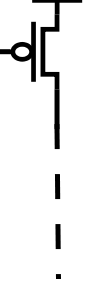
\includegraphics[width=0.12\textwidth] {../fig/hfdst-last-loadtypesswitch.png} \label{fig:switchload}}}
  \subfloat[De bias load]{\makebox[.22\textwidth]{ 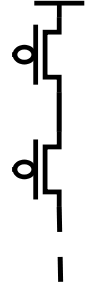
\includegraphics[width=0.12\textwidth] {../fig/hfdst-last-loadtypesbias.png} \label{fig:biasload}}}
  \subfloat[De diode load]{\makebox[.22\textwidth]{ 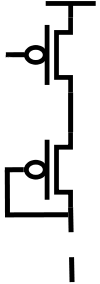
\includegraphics[width=0.12\textwidth] {../fig/hfdst-last-loadtypesdiode.png} \label{fig:diodeload}}}
  \subfloat[De bulk load]{\makebox[.22\textwidth]{ 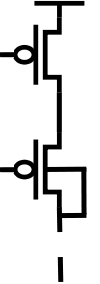
\includegraphics[width=0.12\textwidth] {../fig/hfdst-last-loadtypesbulk.png} \label{fig:bulkload}}}
  \caption{De verschillende types lastimpedanties}
  \label{fig:loads}
\end{figure}

\subsection{Lineaire sweep op de lasten}\label{sec:linload}
\paragraph{}
De switchload bestaat uit \'{e}\'{e}n pMOS-transistor die volledig wordt aan- of afgesloten. Een lineare sweep met een transistorbreedte tussen 100nm en 500nm werd uitgevoerd en is geïllustreerd in figuur \ref{fig:switchloadsim}. Bij het vergroten van de transistorbreedte zal de aanweerstand dalen en het verschil tussen de BL-spanninen ook. Als we deze last vergelijken met het simpele model uit sectie \ref{sec:simplemodel}, zit de weerstandswaarde aan de linker kant van de piek uit figuur \ref{fig:rpiek}. Bij het vergroten van de transistorbreedte zal de BL-spanning stijgen en de spanningsval over het geheugenelement dus ook. Verder volgt de settling-tijd ook het simpele model uit sectie \ref{sec:simplemodel}, waarbij de settling-tijd daalt bij kleinere weerstandswaardes.

\paragraph{}
De biasload, is een last met twee pMOS-transistoren in serie. De bovenste transistor wordt als een schakelaar gebruikt en dus volledig aan- of afgesloten. De onderste transistor wordt gebiased op een bepaalde spanning. Het voordeel van de biasload is dat men een grotere weerstand kan maken en dus de piek kan bereiken uit figuur \ref{fig:rpiek}. Dit kan men duidelijk zien op de x-assen van figuur \ref{fig:biasloadsim}. Ook hier zijn de breedtes van de transistoren gesweeept tussen 100nm en 500nm. De biasspanning is tussen 0V en 0.4V gesweept. Een hogere biasspanning heeft geen nuttige bijdrage. Omdat de kleinste weerstand die deze configuratie kan aannemen binnen deze sweeprange net iets groter is als deze van de switchload, is de biasload ook iets trager. De oplossingen waarbij dit het geval is, hebben echter een onbruikbaar verschill in BL-spanningen. De spanningsval over het geheugenelement is vergeleken met de switchload heel wat hoger maar voor de meeste oplossingen ligt ze nog steeds onder de limiet van 0.5V.

\paragraph{}
De diodeload bestaat ook uit twee transistoren, de bovenste functioneert zoals de biasload als schakelaar. Bij de onderste transistor zijn drain en gate kortgesloten, dit noemt men een diode-geconnecteerde MOS-transistor. Uit de resultaten van de sweep (figuur \ref{fig:diodeloadsim}) blijkt dat de settling met deze last heel snel is, maar het BL-spanningsverschil is te klein om bruikbaar te zijn.

\paragraph{}
De bulkload werd voorgesteld in de paper van Ren et al. \cite{bulkload} als een goede kandidaat omwille van zijn grote uitgangsimpedantie. Deze last bestaat uit een schakelaartransistor en een bulk-geconnecteerde transistor. Deze bulk-geconnecteerde transistor wordt op 0V gebiased aangezien dit de beste resultaten gaf. De breedtes van de transistoren zijn gesweept tussen 100nm en 500nm. De resultaten van deze sweep zijn geïllustreerd in figuur \ref{fig:bulkloadsim}. In de resultaten kan gezien worden dat deze last zich vergelijkbaar gedraagd als de biasload. Enkel op het vlak van settling-tijd zijn er oplossingen die beter zijn.

\afterpage{
\begin{figure}
  \centering
  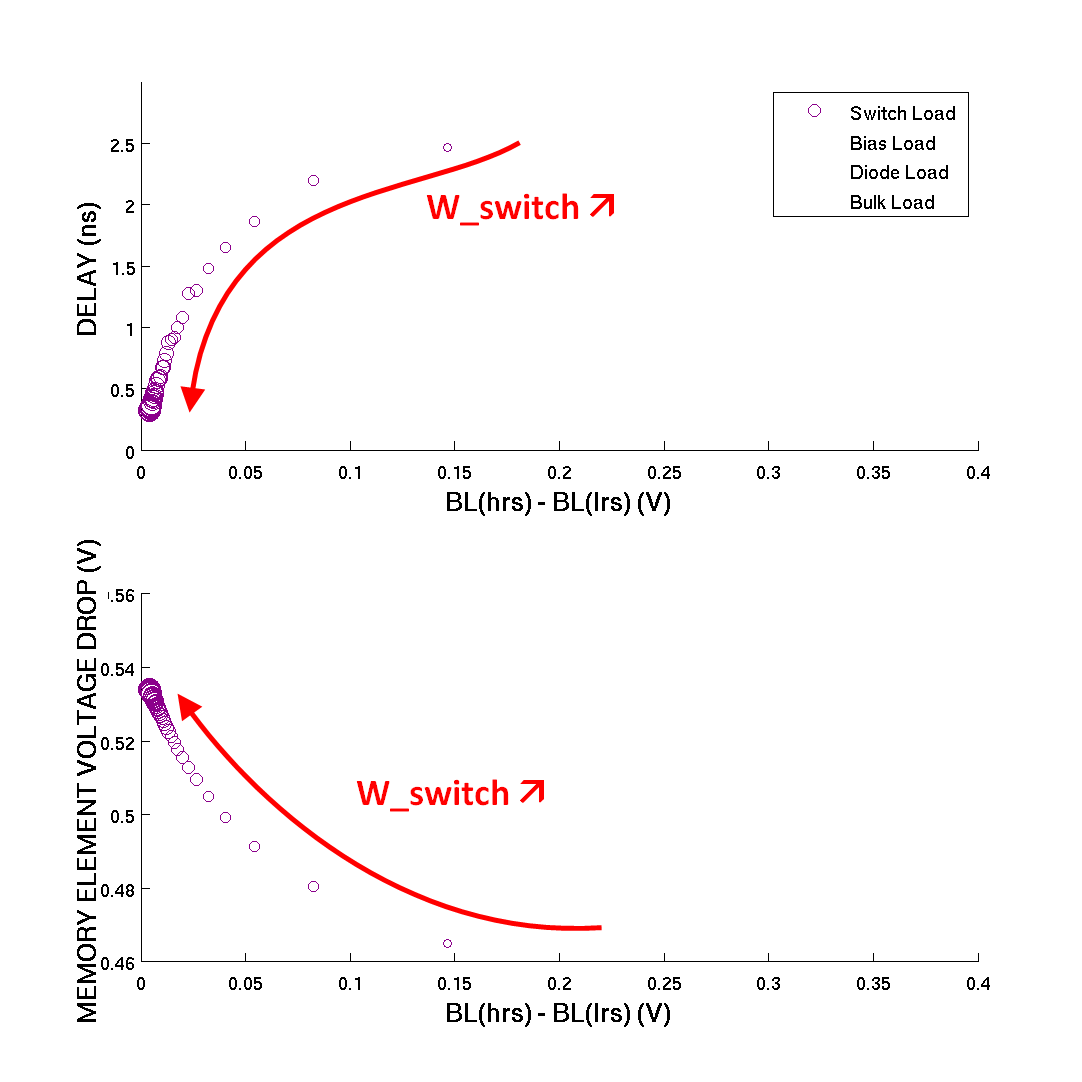
\includegraphics[width=0.67\textwidth]{../fig/hfdst-last-switchload.png}
  \caption{Lineaire sweep van switchload}
  \label{fig:switchloadsim}
 \centering
  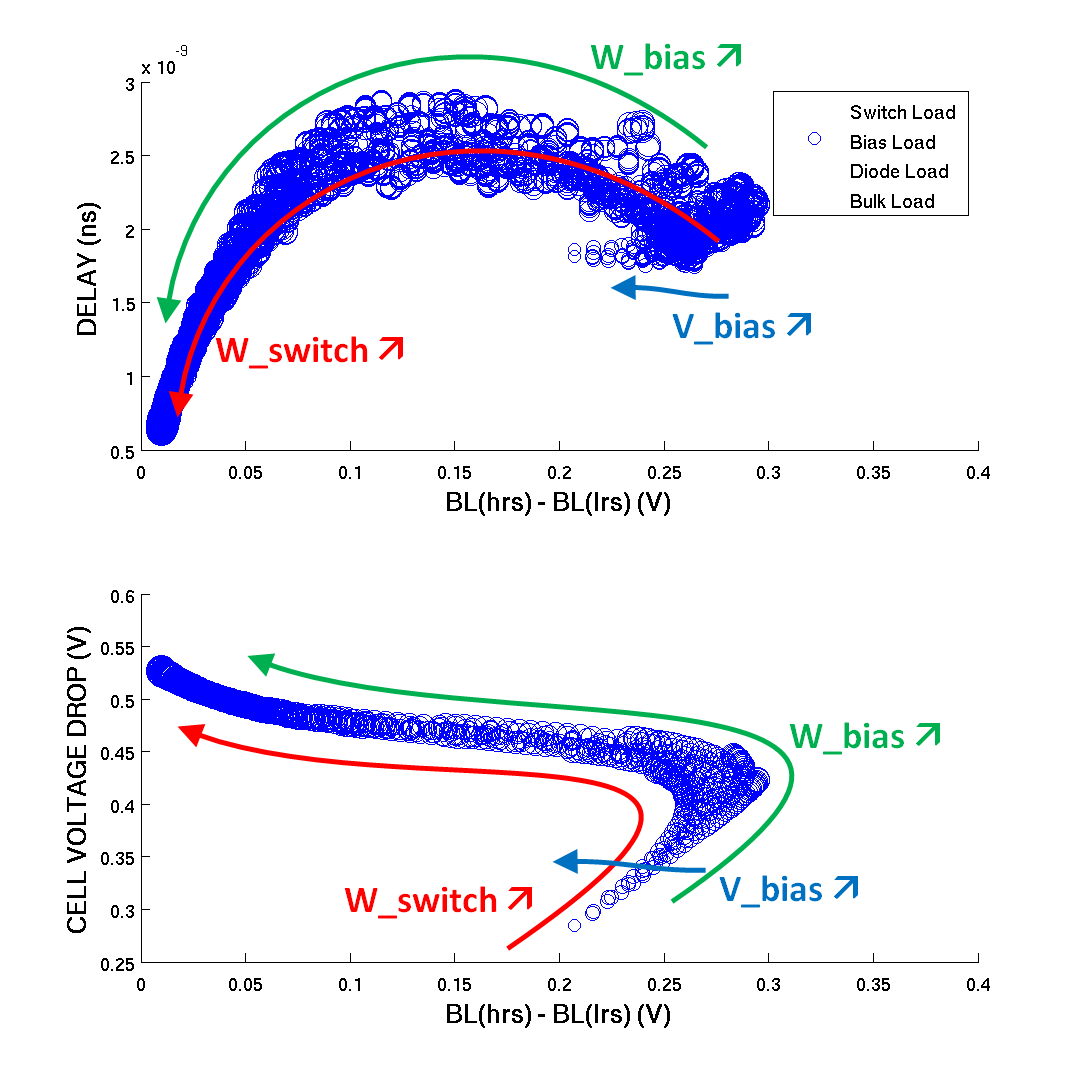
\includegraphics[width=0.67\textwidth]{../fig/hfdst-last-biasload.png}
  \caption{Lineaire sweep van biasload}
  \label{fig:biasloadsim}
\end{figure}
}
\afterpage{
\begin{figure}
  \centering
  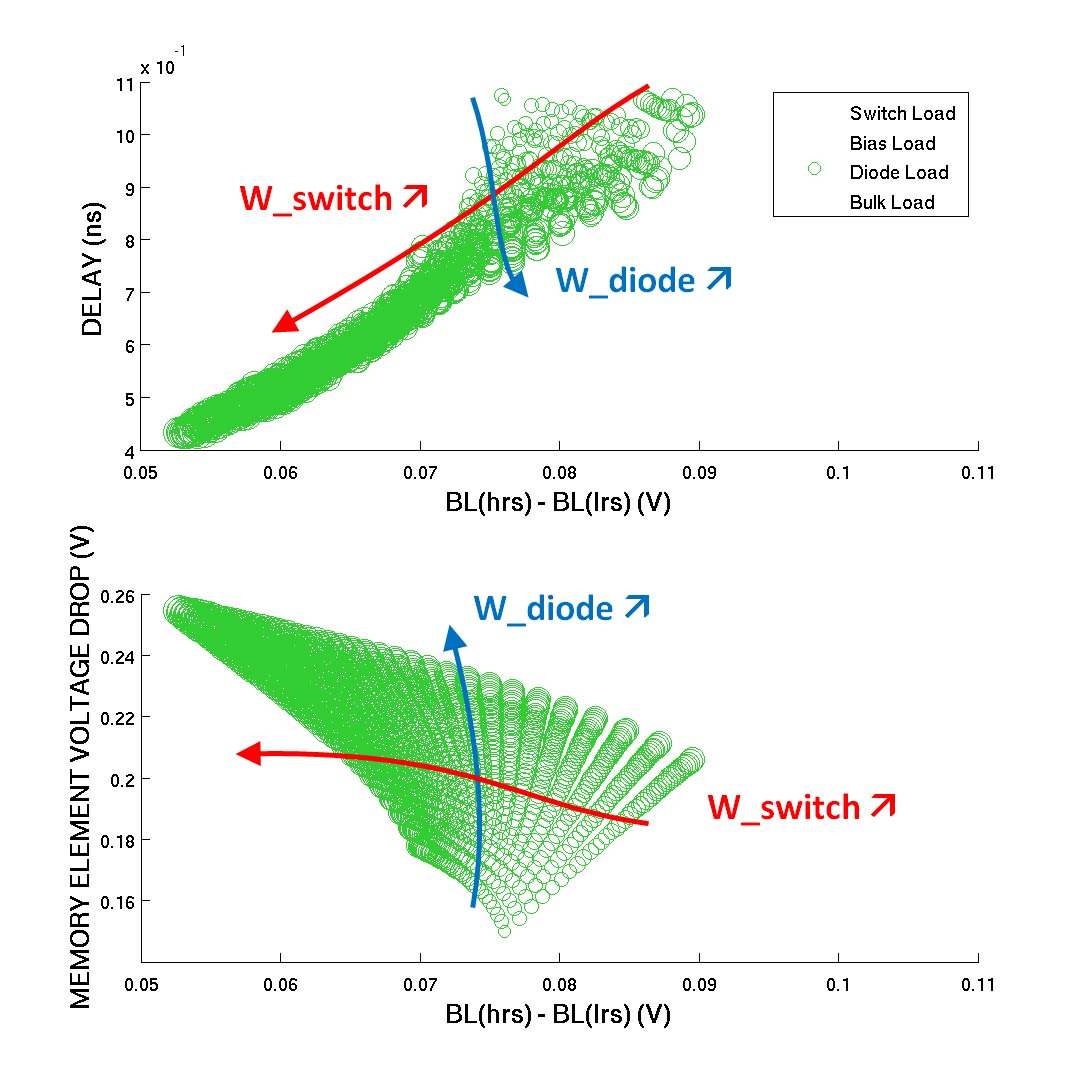
\includegraphics[width=0.67\textwidth]{../fig/hfdst-last-diodeload.png}
  \caption{Lineaire sweep van diodeload}
  \label{fig:diodeloadsim}
  \centering
  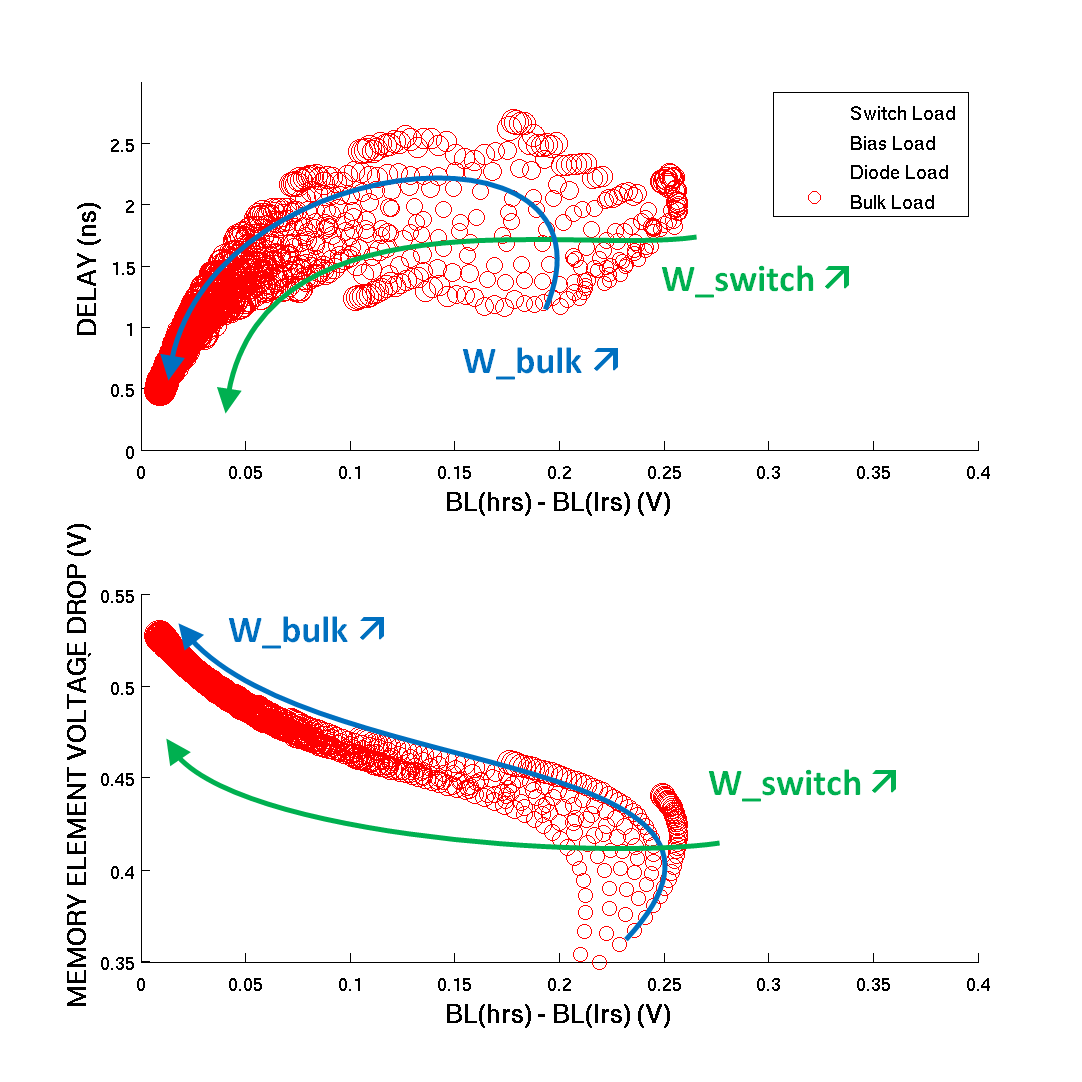
\includegraphics[width=0.67\textwidth]{../fig/hfdst-last-bulkload.png}
  \caption{Lineaire sweep van bulkload}
  \label{fig:bulkloadsim}
\end{figure}
}

\subsection{Het toevoegen van variabiliteit}\label{sec:varload}
Na een selectie te hebben gemaakt van de oplossingen uit de vorige sectie, worden met deze oplossingen nieuwe simulaties gedaan waarbij er variabiliteit is toegevoegd. De variabiliteit is toegevoegd op alle transistoren in het testcircuit en op de weerstandswaarde van de geheugenelementen. Voor de transistoren wordt er een Pelgrom constante voor Vt van $2.5mV\mu m$ gebruikt en voor $\beta$ een van $1.2\mu m$\cite{ppt:variatie}. Voor de weerstandswaarde van de memristors wordt er een gaussische verdeling gebruikt met verwachtingswaardes 7.5k$\Omega$ en 32.5k$\Omega$ en met $\sigma = 0.833k\Omega$. Er worden telkens 500 Monte Carlo simulaties uitgevoerd per oplossing. Hierna worden de BL-spanningen van cellen met een HRS en LRS gefit op een gaussische distributie. De oplossing met het grootste BL-spanningsverschil tussen de extrema van HRS en LRS is een biasload met een schakelaartransistorbreedte van 100nm, een biastransistorbreedte van 180nm en een biasspanning van 0V. De BL-spanning-distributies zijn geïllustreerd op figuur \ref{fig:distbias}. Uit de CDF van deze verdelingen kan men besluiten dat het BL-spanningsverschil in $99.9^2\%$ van de gevallen\footnote{$CDF(V_{BL-RHS})<0,1\%-CDF(V_{BL-LHS})>99,9\%$} groter zal zijn dan 65mV. Dit is niet bijzonder veel aangezien de distributie van de referentiespanning hier ook tussen moet passen en er daarna nog marge moet zijn voor de offsetspanning van de sense amplifier. De invloed van de variabiliteit op de transistoren in de last is even groot voor beide transistoren. (??????????)

\begin{figure}[!ht]
  \centering
  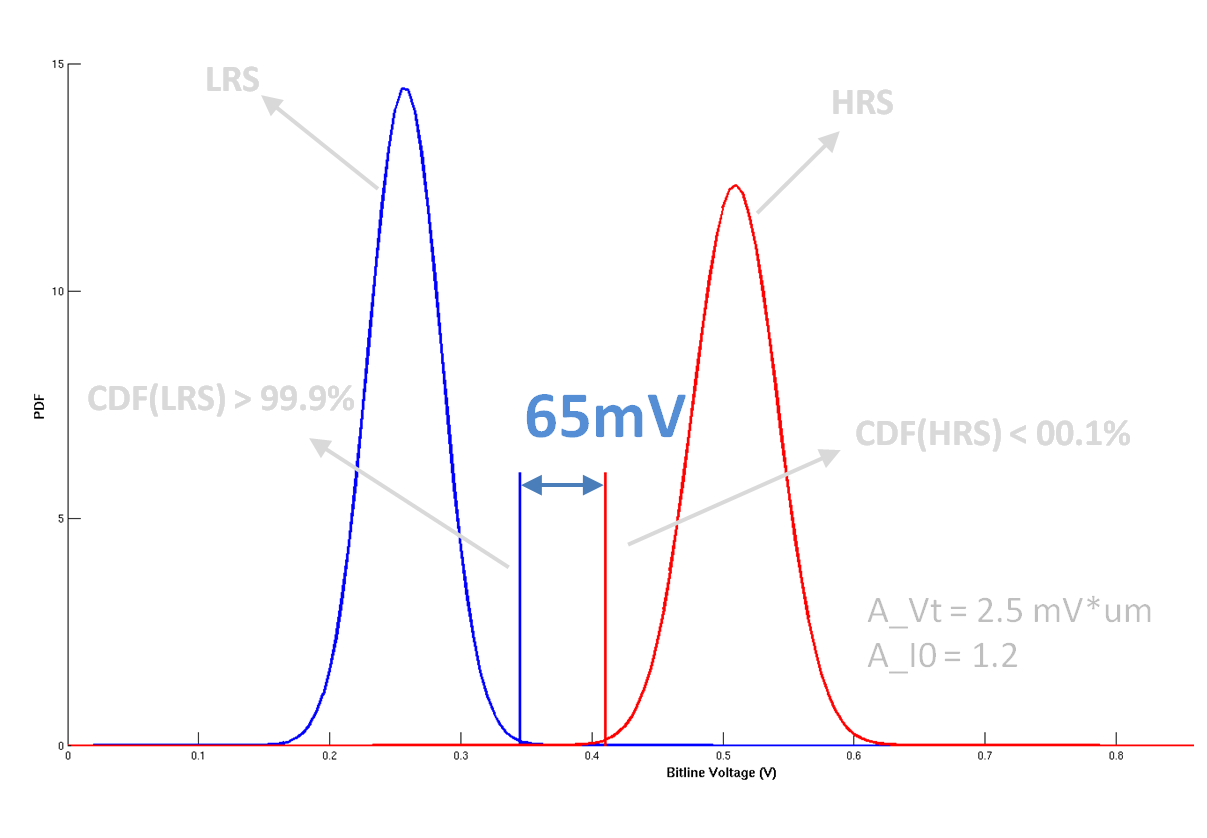
\includegraphics[width=0.67\textwidth]{../fig/hfdst-last-var1.png}
  \caption{BL-spanningsverdeling voor een biasload}
  \label{fig:distbias}
\end{figure}

Figuur \ref{fig:distref} stelt de distributie van de referentiespanning voor. De verschillende curves stellen referentiesignalen opgewekt met meerdere referentiecellen [bereik 2 tot 30, steeds evenveel LRS- als HRS-cellen] voor. Zoals gezien kan worden, heeft men een groot aantal cellen nodig om een distributie breedte van 39mV te krijgen. Dit betekent dat de offsetspanning van de SA niet groter mag zijn dan 10mV, indien de vooraf vermelde biasload gebruikt wordt. Dit is een zeer strenge voorwaarde. Daarom wordt de constraint waarbij de transistorlengte minimaal gehouden wordt, opgeheven in de volgende sectie.

\begin{figure}[!ht]
  \centering
  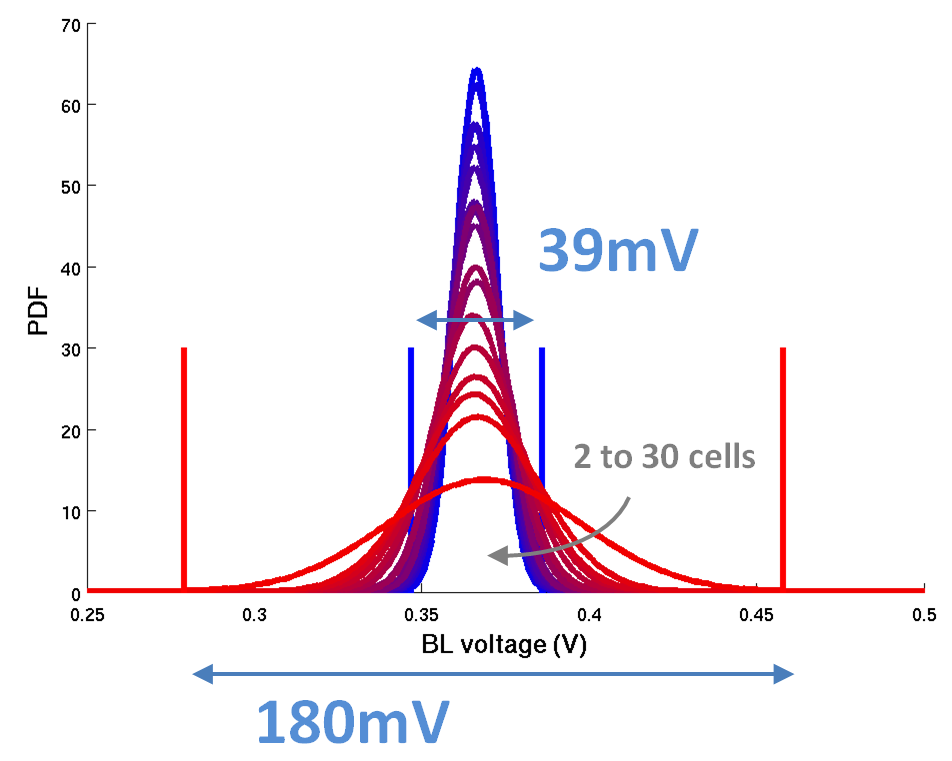
\includegraphics[width=0.67\textwidth]{../fig/hfdst-last-ref.png}
  \caption{Lineaire sweep van switchload}
  \label{fig:distref}
\end{figure}


\subsection{De transistor lengte vergroten}\label{sec:finaleload}
Om de variabiliteit onder controle te houden moeten de transistoren vergroot worden. Twee opties worden hiervoor overwogen. De eerste is het toevoegen van een derde transistor in serie. Om dezelfde lastimpedantie te bekomen als voor 2 transistoren in serie, moeten de drie transistoren een grote breedte hebben. De $\frac{W}{L}$-verhouding vergroten, verlaagt de aanweerstand van de individuele transistoren, maar door ze in serie te schakelen blijft de equivalente weerstand voldoende groot. Omwille van de vergrote afmetingen zouden ze bovendien minder gevoelig zijn voor mismatch. Hierbij wordt wel verondersteld dat alle drie de transistoren zich in lineair bevinden. In werkelijkheid blijkt de onderste transistor zich in near- tot sub-threshold te bevinden. De stroom in het sub-theshold gebied varieert exponentieel met $V_{GS}-V_{T}$. De stroom en aanweerstand van de transistor zijn dus zeer gevoelig voor VT-variaties. Dit fenomeen ziet men niet bij 2 transistoren in serie, aangezien de transistoren hier in het lineare gebied zijn. Daarom wordt er om de mismatch onder controle te houden geopteerd voor de tweede optie, namelijk het vergroten van de transistorlengte. De lengte vergroten resulteert in een toename van de aanweerstand en vermindert variabiliteit. Omwille van eenvoudigheid, wordt er met deze nieuwe ontwerpkeuze teruggegrepen naar de switchload.\\
Figuur \ref{fig:length} geeft de resultaten weer van een sweep van verschillende lengtes en breedtes voor een switchload. De resultaten worden voorgesteld in functie van $\frac{W}{L}$ wat een indicatie is voor de weerstand van de transistor. In de bovenste figuur kan men duidelijk een maximum zien voor het verschil in BL-spanning zoals in sectie \ref{sec:simplemodel} werd voorspeld. Verder dient worden opgemerkt dat er best een oplossing aan de linkerkant van het maximum gekozen wordt aangezien de spanningsval over het geheugenelement van de oplossingen aan de rechterkant van het maximum te hoog zijn.
\begin{figure}[!ht]
  \centering
  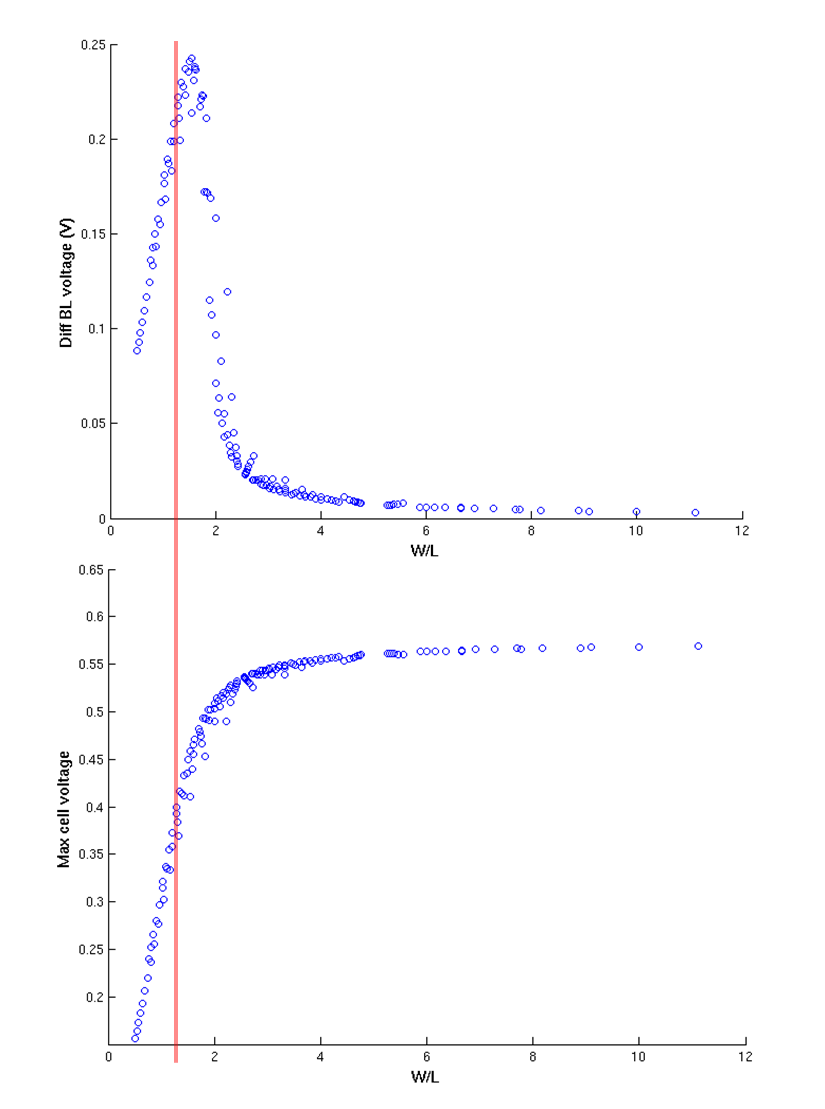
\includegraphics[width=0.66\textwidth]{../fig/hfdst-last-length.png}
  \caption{Verschillende oplossingen voor de switchload met variabele lengtes en breedtes}
  \label{fig:length}
\end{figure}

Voor de finale last wordt er geopteerd voor een transistor met lengte gelijk aan 198nm en breedte gelijk aan 300nm. Op figuur \ref{fig:length} wordt deze aangeduid met de rode lijn. Op figuur \ref{fig:distswitch} wordt de BL-spanningsdistributie van deze last getoond. Het minimale verschil in BL-spanning is bijna 200mV. De distributie van het referentiesignaal is ook aangegeven op deze figuur. De referentie bestaat uit 4 referentie cellen waarvan 2 in HRS en 2 in LRS. Opvallend is dat deze referentie niet in het centrum zit tussen de BL-spanningen. Dit kan opgelost worden door een niet gelijk aantal referentiecellen in HRS en LRS voor het referentiesignaal te gebruiken. Aangezien de standaarddeviatie op de BL-spanningen heel wat beter is, kan er gerust gekozen worden voor een last met een kleiner nominaal BL-spanningsverschil \label{anderelast}. Dit kan 2 voordelen met zich mee brengen. Zo is de spanningsval van de memristor lager wanneer men een last kiest links van het maximum in figuur \ref{fig:length}. Voor dergelijke lastimpedanties moeten de BLs bovendien tot een lagere spanning opladen wat een energie winst oplevert. Ondanks deze voordelen werd er toch geopteerd voor de oplossing met het grootste BL-spanningsverschil.

\begin{figure}[!ht]
  \centering
  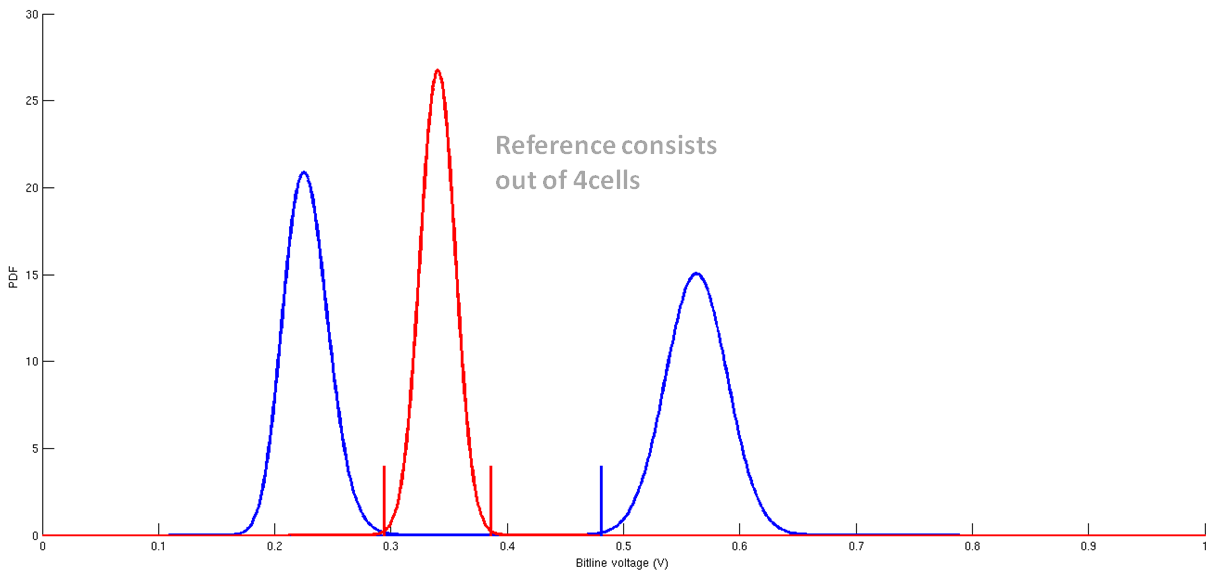
\includegraphics[width=0.67\textwidth]{../fig/hfdst-last-var2.png}
  \caption{BL-spanningsverdeling voor de finale lastimpedantie}
  \label{fig:distswitch}
\end{figure}

\section{Besluit}
Verschillende kandidaten voor lastimpedanties werden overwogen. Aanvankelijk werd er getracht een last met minimale transistorlengtes te vinden, dit bleek echter niet haalbaar wanneer variabiliteit in rekening wordt genomen. Een enkele transitor met niet-minimale afmetingen bleek de beste resultaten te leveren wat betreft BL-spanningsverschil en spanningsval over geheugenelement.